 \documentclass[12pt]{article}
 
\usepackage[margin=1in]{geometry}
\usepackage{amsmath,amsthm,amssymb}
\usepackage{mathtools}
\usepackage{booktabs}
\usepackage{multirow}
\usepackage{graphicx}
%\graphicspath{{/}}
\newcommand{\N}{\mathbb{N}}
\newcommand{\R}{\mathbb{R}}
\newcommand{\Z}{\mathbb{Z}}
\newcommand{\Q}{\mathbb{Q}}

\newenvironment{problem}[2][Problem]{\begin{trivlist}
\item[\hskip \labelsep {\bfseries #1}\hskip \labelsep {\bfseries #2}]}{\end{trivlist}}
\newenvironment{exercise}[2][Exercise]{\begin{trivlist}
\item[\hskip \labelsep {\small\bfseries #1}\hskip \labelsep {\small\bfseries #2}]}{\end{trivlist}}
\newenvironment{epart}[2][Part]{\begin{trivlist}
\item[\hskip \labelsep {\footnotesize\bfseries #1}\hskip \labelsep {\footnotesize\bfseries #2}]}{\end{trivlist}}

\DeclarePairedDelimiter\abs{\lvert}{\rvert}
\DeclarePairedDelimiter\norm{\lVert}{\rVert}

\makeatletter
\let\oldabs\abs
\def\abs{\@ifstar{\oldabs}{\oldabs*}}

\let\oldnorm\norm
\def\norm{\@ifstar{\oldnorm}{\oldnorm*}}
\makeatother

\DeclarePairedDelimiter\ceil{\lceil}{\rceil}
\DeclarePairedDelimiter\floor{\lfloor}{\rfloor}

\newtheorem{theorem}{Theorem}[section]
\newtheorem{corollary}{Corollary}[theorem]
\newtheorem{lemma}[theorem]{Lemma}
 
\begin{document}
 
\title{MAT 128B Project 2}
\author{Steven An, Kyle Cox}
\date{March 14, 2018}
\maketitle

\subsection*{Distribution of work}
Rather than divvying up the work, Steven and Kyle met in person and discussed the project. For efficiency they at times worked on different sections. Steven began the report while Kyle set up the GitHub repository (https://github.com/KyleDCox/128B\_project2), did parts i, ii, and set up the main program. Following, Steven wrote parts iii and v, while Kyle worked on iv. However, throughout these periods there was consistent communication and idea-bouncing. Together, they decoded the prompt and interpreted how to conquer each section. As they worked, they had to decide how each of the parts would connect - choosing appropriate objects and methods took deliberation on their part.


At times, while brainstorming particularly challenging tasks, the two worked through the problems by hand and compared their results. Kyle wrote the initial framework for part vi, and in moving toward generating part vii, the two had to go back and debug each of the parts. Debugging was mostly discussed in person and resolved by both Steven and Kyle. When taking breaks between meeting, some work and debugging was done remotely by each person.


Steven's computer was able to run the program much faster than Kyle's machine. As such, much of the computation in part vii was taken on by Steven. The two worked on part vii together, deciding how to best test their network against a variety of parameter regimes. The two had to debug this section of the code for some time in order to get the training to work. Ultimately, Steven was able to debug part vii and run it many times for statistical analysis between different parameter regimes.


The report was written by both Steven and Kyle with communication about revisions and additions.

\subsection*{Part (i)}
Followed instructions.

\subsection*{Part (ii)}
Done as requested.  
See Supplementary Figures.

\subsection*{Part (iii)}
Let $x$ be $NET$.
We have 
\[OUT = F(x) = \frac{1}{1+e^{-x}}\]
and
\[F^\prime(x) = \frac{e^{-x}}{(1+e^{-x})^2} = \frac{1-1+e^{-x}}{(1+e^{-x})^2} = \frac{1+e^{-x}}{(1+e^{-x})^2} -\frac{1}{(1+e^{-x})^2} = F(x)(1-F(x))\]
which was to be shown.
When $x$ is large and positive, then $F(x)$ will be close to 1 because as $x\rightarrow\infty$, $e^{-x}\rightarrow 0$.
On the other hand, when $x$ is large and negative, $F(x)$ will tend to zero.
This is because $e^{-x}$ is very large when $x\ll 0$.
Therefore, as the numerator is constant, $F(x)$ will tend to zero.
Another example of a function that can be used is $-\arctan\left(x\right) + \pi/2$.
The function is both differentiable and uniformly bounded.
However, here, when $x$ is negative, the function approaches its upper bound and \textit{vice versa}.
The relation between the input and output need not be standard.
One may consider sinusoidal functions like $\sin(x)+1 \text{ and }\cos(x)+1$.
These are bounded, differentiable, and always positive, but are oscillatory.
For strictly monotonic functions, either $F$ approaches its lower or upper bound when $x$ is large and positive and \textit{vice versa}.
\subsection*{Part (iv)}
This function returns a matrix that contains the value of the neurons at each neural network for each layer except for the input layer.
This is manually done for the first hidden layer because the first set of weights is not in the three dimensional array.
The appropriate matrices and neuron values are chosen, put as arguments into the function from part (iii) and the results recorded.

\subsection*{Part (v)}
This function creates the weights of the connections between layers.
On the advice of a friend, values of the weights were chosen to be distributed on the interval [-0.01, 0.01].
To save memory, the matrix of weights going from the input layer to the first hidden layer has its own matrix.
For all other layers, there is a three dimension matrix where each layer stores the weights between each layer.
For our weight matrix $W\in\R^{m\times n\times k}$, $w_{ijk}$ is the weight from the $j^{th}$ node of the $k^{th}$ hidden layer to the $i^{th}$ node of the $(k+1)^{th}$ hidden layer. We consider our output layer as the last hidden layer in reference to this matrix.
This allows for less confusing notation in part (iv).
$NumHidden$ is the number of hidden layers.
$NumNeurons$ is a vector containing the number of neurons in each respective hidden layer (not including our output layer).
The length of $NumNeurons$ is $NumHidden+1$ because the number of neurons in the output layer is 10 and there must be weights going to the output layer.
The range of weights is the same as before.
\subsection*{Part (vi)}
The forward propagation is done with a call to the function in part (iv).
It should be noted that the error computation with the update of 
weights as described in the prompt is incorrect.
This was verified by the fact that every neural network we generated from those instructions failing to confirm a single digit when only trained for that digit.
Therefore, we chose to compute $ERROR=TARGET-OUTPUT$ where \emph{TARGET}, for the $(i-1)^\text{th}$, is the standard basis vector, $e_i$.
We keep the original weight update equation, as now there are signs.
Before, if there was an error, and the output of the neural network was too high, all that would happen is that the weights would increase.
The $\delta$ vector is computed all at once.
here, $OUT_k$ is the output layer.
This is done by \[\delta = OUT_k \circ (1-OUT_k) \circ ERROR\]
where $\circ$ is the Hadamard product.
Then, the matrix is \[\Delta w_k = \eta \cdot \delta \cdot OUT_{k-1}^T.\]
NOTE: The weight change matrix is the \textbf{transpose} of what is described in the prompt.  
This is because we chose to implement the transpose of the weight matrix.

We first note that the index of summation for the $\delta$ computation in the hidden layer weight adjustment is $q$ and not $k$ as typed.
Then, it is clear that the first part of the multiplication is $O_j\circ (I-O_j)$.
It shall now be shown that the expression provided is incorrect.
The sum we'd like to convert to matrix form for the $k^{th}$ layer is 
\[\sum_{q}\delta_q w_{pq}.\]
Let $D_k$ be all $\delta$'s for layer k.
That is, for row $p$ of matrix $W$, multiply the $q^{th}$ element of $\delta$ to the element in the $q^{th}$ column (and $p^{th}$ row of $W$.
So the corresponding expression is $(W\delta)_p$, the $p^{th}$ element of that vector.
Then, for the general case, we have \[D_j = WD_k \circ O_j\circ (I-O_j)\]
where $I$ is the column vector of ones (as used in the prompt).
Since the weight matrix for our program is $\hat W =W^T$, the implementation found is actually 
\[D_j = (D_k^T\hat W)^T\circ O_j\circ (I-O_j).\]
Then, the same equation as above is used to compute \(\Delta w\).

\subsection*{Part (vii)}
To train our network, we run ever image through the network, a different digit every iteration, and perform the reverse pass.
In order to eliminate bias, the same amount of images for each digit was used.

To check if the neural net guesses the correct digit, we check to see if the position of the max element of the output layer is equal to $1+\text{the correct digit}$ (because positioning in matlab begins at 1, but our digits begin at 0). 
If this is true, then we add one to our count of correct guesses, then divide the total number of correct guesses by the total number of test inputs.

After training the system we first tested a regime of two hidden layer with 100 and 50 neurons respectively. 
We denote this as `100 - 50, 5421x10' where the second term is the number of images from each digit that was used for training.
This network structure was tested by varying the number of training iterations (one iteration is training through the entire training set once). 
We tested this 20 times for 10 iterations and 15 iterations each, and once for 20 iterations (as the latter took too much time).

It should be said that in general, the higher the iteration count, the smaller the error.
However, if the neural network becomes overfitted to the training data, the error percentage rises.
It is surmised that with 20 iterations, the neural network becomes overfitted to the training data and thus has a lower success rate with the test data. 

The results are provided in the tables below. 
The Training Error \% denotes the percent of the time the neural net guesses the incorrect digit when the training set is used as an input. 
Similarly, Test Error \% represents the same for when the test set is used as an input.

\begin{table}[h]
	\begin{center}
		\caption{Error Stats for 100 - 50, 5421x10}
		\label{tab:table1}
		\begin{tabular}{|c|c|c|c|c|c|c|c|c|}
			\hline
			\multirow{2}{*}\textbf{Iterations} & \multicolumn{4}{c|}{\textbf{Training Error \%}} &  \multicolumn{4}{c|}{\textbf{Test Error\%}} \\
			\cline{2-9}
			&Min & Mean & Max & Variance & Min & Mean & Max& Variance\\
			\hline
			10 & 3.99 & 5.67 & 7.35 & 0.818 & 4.7 & 6.41 & 8.53 & 0.947\\
			\hline
			15 & 2.94 & 3.95 & 6.51 & 0.641 & 4.22 & 5.13 & 6.61 & 0.314 \\
			\hline
			20 & N/a & 2.7 & N/a & N/a & N/a & 6.08 & N/a & N/a\\
			\hline
		\end{tabular}
	\end{center}
\end{table}

We see that from our results of training the neural network with 10 iterations 20 times that indeed, all aspects of error decreased.
For this network structure, the value of $\eta$ did not really matter because multiple values were tested before these 41 tests were run and the error rate were not very different from the ones seen here.

\begin{table}[h]
	\begin{center}
		\caption{Error Stats for 50 - 25, 5421x10}
		\label{tab:table1}
		\begin{tabular}{|c|c|c|c|c|c|c|c|c|}
			\hline
			\multirow{2}{*}\textbf{Iterations} & \multicolumn{4}{c|}{\textbf{Training Error \%}} &  \multicolumn{4}{c|}{\textbf{Test Error\%}} \\
			\cline{2-9}
			&Min & Mean & Max & Variance & Min & Mean & Max& Variance\\
			\hline
			10 & 4.89 & 22.43 & 69.54 & 488.41 & 5.82 & 22.97 & 69.32 & 479.61\\
			\hline
			15 & 3.71 & 6.89 & 20.41 & 19.9 & 4.61 &7.77 & 20.23 & 18.38\\
			\hline
			20 & N/a & 3.41 & N/a & N/a & N/a & 5.0 & N/a & N/a\\
			\hline
		\end{tabular}
	\end{center}
\end{table}

For this structure, we see that the decrease in neurons negatively affected the success rate.
Even though the best result was close to that of the 100 - 50 structure, the variance was orders higher for 10 and 15 iterations.
Perhaps there is a balance between training the network and not over-training it.
The boundary between the two, would, in our speculations, be unknowable because we do not fully understand how the sigmoid function and weights represent the network's cognition, if it has any.
Regardless, our original claim of error decreasing as training iterations increase is further corroborated by this smaller neural network.

Another hypothesis is that because the neuron count in the first layer is so low, it cannot faithfully represent the `essence' of the digits.
That is, what the neural network represents is too convoluted and  certain properties of the digit cannot be easily assigned to the representation given by the network.
This `bad fitting' of the digits is what contributes to the low accuracy (as compared to 100 50).

The value of $\eta$ did matter for some sets of initial weights when training this network.
For certain weights, if $\eta = 0.01$, then it would only train for the last digit, 9.
This was further supported by testing how the network performed when it was only trained and tested on two digits.
Even for two digits, the network would only be trained for the second one.
Choosing $\eta = 0.025$ fixed the problem and generated the results seen.

\begin{table}[h]
	\begin{center}
		\caption{Error Stats for 100 - 50, 2710x10}
		\label{tab:table1}
		\begin{tabular}{|c|c|c|c|c|c|c|c|c|}
			\hline
			\multirow{2}{*}\textbf{Iterations} & \multicolumn{4}{c|}{\textbf{Training Error \%}} &  \multicolumn{4}{c|}{\textbf{Test Error\%}} \\
			\cline{2-9}
			&Min & Mean & Max & Variance & Min & Mean & Max& Variance\\
			\hline
			10 & 17.3 & 20.37 & 22.46 & 2.23 & 14.99 & 18.31 & 22.11 & 4.51\\
			\hline
			15 & 17.26 & 19.25 & 21.64 & 1.68 & 14.59 &16.21 & 19.23 & 1.42 \\
			\hline
			20 & N/a & 18.45 & N/a & N/a & N/a & 15.17 & N/a & N/a\\
			\hline
		\end{tabular}
	\end{center}
\end{table}

Holding the other variables constant, changing the training set into one with less images results in the loss of accuracy of the neural network.
We see that the variance increased along with the minimum, mean and maximum.
This gives us evidence that there is a minimum amount of sample images that need to be used as the neural network's efficacy has decreased by a considerable amount.
An explanation could be that by having less images, the set of digits were less diverse and the neural network in its training was lacking information.

\begin{table}[h]
	\begin{center}
		\caption{Error Stats for 50 - 25, 2710x10}
		\label{tab:table1}
		\begin{tabular}{|c|c|c|c|c|c|c|c|c|}
			\hline
			\multirow{2}{*}\textbf{Iterations} & \multicolumn{4}{c|}{\textbf{Training Error \%}} &  \multicolumn{4}{c|}{\textbf{Test Error\%}} \\
			\cline{2-9}
			&Min & Mean & Max & Variance & Min & Mean & Max& Variance\\
			\hline
			10 & 40.75 & 62.66 & 90.09 & 212.86 & 43.85 & 63.93 & 89.91 & 188.89\\
			\hline
			15 & 18.59 & 45.65 & 90.09 & 532.38 & 21.24 & 46.21 & 89.91 & 547.77 \\
			\hline
			20 & N/a & 21.78 & N/a & N/a & N/a & 20.03 & N/a & N/a\\
			\hline
		\end{tabular}
	\end{center}
\end{table}

The results here show that having two hidden layeres with 100 and 50 neurons is a much more stable network than 50 and 25 neurons.
In three of the twenty networks created, the weights were such that it could only correctly identify one digit, leading to the 90 percent error rate.
All semblance of `good performance' from the neural network (when it had 5421 images per digit) was lost.
The error rate skyrocketed and the network could not be improved by much.

\begin{table}[h]
	\begin{center}
		\caption{Error for 100 - 50 - 25, 5421x10}
		\label{tab:table2}
		\begin{tabular}{|c|c|c|}
			\hline
			\textbf{Iterations} & \textbf{Training Error \%} & \textbf{Test Error \%} \\
			\hline
			10 & 23.97 & 18.30\\
			& 25.99 & 22.88\\
			\hline
			20 & 20.14 & 16.52 \\
			\hline
		\end{tabular}
	\end{center}
\end{table}

The neural network was trained with ten iterations, giving the result in the first row.
Then, the same set of weights was trained again to get the result in the third row.
It might be claimed that the more neurons the network has, the better it will be performed.
These results do no give credence to either view for one can claim that if the network were further trained, the accuracy would increase to the mid nineties, but skeptics may say that the network structure inherently guarantees that the accuracy will not be high.
Since we do not know the rate of convergence to the truth for the network, not much can be drawn from the small increase in accuracy when the training set was run through ten more times.  
We think it would be a waste of time to test this for smaller training set based on the previous results.

\subsection*{Concluding Remarks}

We have seen now that having two hidden layers with 100 and 50 neurons is the best network structure (of those which we tested).
Furthermore, using as many images as possible (in terms of what we have) yielded the best performance.
Empirical results give credence to those claims.
Moreover, for that structure, iterating through the training data set 15 times was found to give the best result. We suppose that increasing training iterations up to a point will increase the accuracy of the neural net; however, after that point any further training will over-train and become accustomed to the training set. Perhaps we could have better trained the network if we were to (for each full training iteration) randomly sort all of the training images, so that there is no structured format or cycle for the training input. This way, perhaps, the net may be more adjusted to receiving random test inputs.


It has also been seen that $\eta$ can determine whether a set of weights with a structure form a good neural network.
However, the effects of changing specific $\eta$ cannot be explained with our data because every time we run the program, a new set of initial weights is generated. We can only observe the results of changing the max-min range of $\eta$. From our understanding of neural nets, these initial weights will place us randomly in the weight-parameter space corresponding to a specific parameter regime. If we consider the error function of our neural net (as a function of each of the weight parameters), then training the neural net moves the neural net down the gradient of the parameter space toward a local minimum. We realize that randomly generating a set of weights determines our initial position within this space. As such, we have little hopes of ever finding the global minimum of our parameter space. Furthermore, we cannot guess how changing our parameter regime (number of layers and number of neurons per layer) would change the global minimum of the respective error function. Perhaps our above tests reveal that some parameter regimes hit poor local minimums most of the time - who is to say that their global minimum is better than our guess for the best parameter regime? We suggest that the quality of a nerual net's setup (those parameters determining the number and size of layers) should be the quality of the net when initialized at a number of random initial weights. That is, perhaps the quality of a neural net has to do with its average local minimum of the weight function. This is why we felt it important to have significant sample sizes for the error analysis above.


Again, these statements are simply suppositions on our part. Putative hypotheses have been given to try and explain why the performance of other structures and iteration counts did not perform as well.
Though these hypotheses may be teleological, they are the best we can come up with given our limited computational power and na\"ive notion of neural networks.

\subsection*{Supplementary Figures}
This section contains the images for part ii. This also contains tables of the raw error percentages computed by generating various neural networks.
We generated the above tables from analysis on the following data.\\

\begin{figure}[h]
	\caption{Random Examples from Training Set}
	\centering
	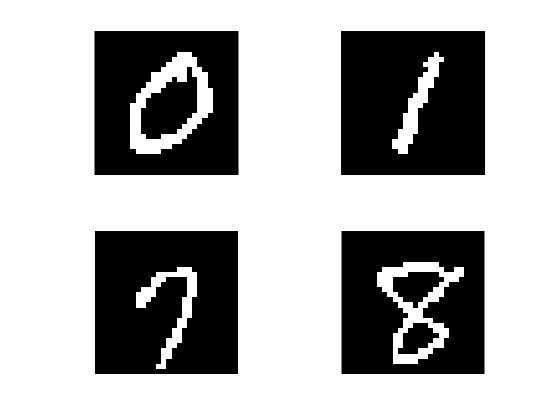
\includegraphics[scale=0.25]{partii_img1.png}
\end{figure}
\begin{figure}
	\caption{Average Images Across All Training Data}
	\centering
	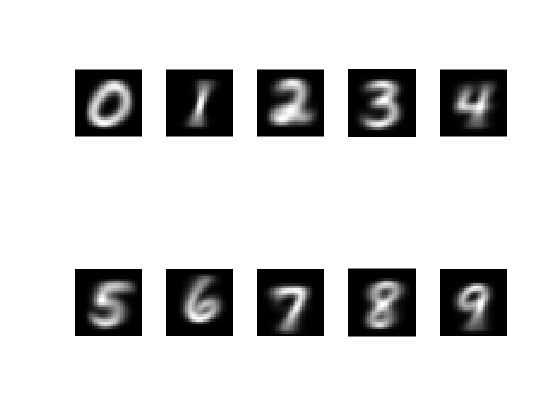
\includegraphics[scale=0.5]{partii_img2.png}
\end{figure}




\begin{table}[h]
	\begin{center}
		\caption{Error for 100 - 50, 5421x10}
		\label{tab:table2}
		\begin{tabular}{|c|c|c|}
			\hline
			\textbf{Iterations} & \textbf{Training Error \%} & \textbf{Test Error \%} \\
			\hline
			10 & 7.35 & 8.53\\
			& 5.81 & 6.9\\
			& 6.17 & 7.2\\
			& 6.11 & 7.43\\
			& 5.53 & 6.47 \\
			& 7.1 & 7.9 \\
			& 4.7 & 5.81 \\
			& 4.45 & 5.03 \\
			& 6.05 & 6.79 \\
			& 6.06 & 6.73 \\
			& 4.67 & 5.45 \\
			& 5.84 & 6.15 \\
			& 5.4 & 6.12 \\
			& 3.99 & 4.7 \\
			& 4.3 & 5.01 \\
			& 5.16 & 5.73 \\
			& 5.96 & 6.32 \\
			& 6.52 & 6.9 \\
			& 5.86 & 6.25 \\
			& 6.42 & 6.81 \\
			\hline
			15 & 3.25 & 5.51\\
			& 3.18 & 5.05\\
			& 3.51 & 5.76\\
			& 5.01 & 5.66\\
			& 3.76 & 4.96\\
			& 4.16 & 5.44\\
			& 3.73 & 4.74\\
			& 3.47 & 4.80\\
			& 2.94 & 4.22\\
			& 3.89 & 5.10\\
			& 4.71 & 5.70\\
			& 4.06 & 5.19\\
			& 3.70 & 4.62\\
			& 3.15 & 4.55\\
			& 3.99 & 5.30\\
			& 4.32 & 5.24\\
			& 3.62 & 4.59\\
			& 4.36 & 5.20\\
			& 6.51 & 6.61\\
			& 3.59 & 4.44\\
			\hline
			20 & 2.7 & 6.08\\
			\hline
		\end{tabular}
	\end{center}
\end{table}

\begin{table}[h]
	\begin{center}
		\caption{Error for 50 - 25, 5421x10}
		\label{tab:table2}
		\begin{tabular}{|c|c|c|}
			\hline
			\textbf{Iterations} & \textbf{Training Error \%} & \textbf{Test Error \%} \\
			\hline
			10 & 12.04 & 11.89\\
			& 4.89 & 5.82\\
			& 6.51 & 6.57\\
			& 5.28 & 5.94\\
			& 52.17 & 52.13\\
			& 30.26 & 30.65\\
			& 47.76 & 47.92\\
			& 6.86 & 7.16\\
			& 7.03 & 7.57\\
			& 7.94 & 8.67\\
			& 8.45 & 8.82\\
			& 69.54 & 69.22\\
			& 6.04 & 6.59\\
			& 8.34 & 8.73\\
			& 69.52 & 69.32\\
			& 7.72 & 7.85\\
			& 6.64 & 6.87\\
			& 33.69 & 34.60\\
			& 13.01 & 13.20\\
			& 47.87 & 47.95\\
			\hline
			15 & 4.21 & 4.96\\
			& 18.12 & 18.30\\
			& 5.84 & 6.72\\
			& 5.95 & 6.93\\
			& 10.29 & 11.15\\
			& 4.92 & 5.76\\
			& 4.02 & 5.35\\
			& 3.72 & 4.61\\
			& 4.48 & 5.49\\
			& 3.71 & 5.04\\
			& 5.34 & 6.64\\
			& 5.99 & 6.93\\
			& 5.25 & 6.37\\
			& 4.84 & 5.86\\
			& 4.13 & 5.31\\
			& 7.99 & 9.10\\
			& 20.41 & 20.23\\
			& 9.44 & 9.69\\
			& 4.16 & 5.39\\
			& 4.89 & 5.62\\
			\hline
			20 & 3.41 & 5.0 \\
			\hline
		\end{tabular}
	\end{center}
\end{table}

\begin{table}[h]
	\begin{center}
		\caption{Error for 100 - 50, 2710x10}
		\label{tab:table2}
		\begin{tabular}{|c|c|c|}
			\hline
			\textbf{Iterations} & \textbf{Training Error \%} & \textbf{Test Error \%} \\
			\hline
			10 & 21.08 & 19.02\\
			& 18.35 & 15.81\\
			& 22.21 & 22.11\\
			& 20.70 & 21.62\\
			& 22.10 & 20.20\\
			& 21.16 & 19.72\\
			& 17.30 & 15.28\\
			& 18.81 & 14.99\\
			& 18.79 & 17.26\\
			& 22.29 & 19.27\\
			& 19.08 & 16.55\\
			& 18.58 & 15.93\\
			& 20.30 & 21.21\\
			& 20.60 & 18.14\\
			& 21.88 & 18.63\\
			& 19.93 & 16.75\\
			& 22.46 & 17.31\\
			& 21.27 & 19.23\\
			& 20.35 & 17.17\\
			& 20.15 & 20.03\\
			\hline
			15 & 18.80 & 15.81\\
			& 17.80 & 14.59\\
			& 19.99 & 16.29\\
			& 21.43 & 16.99\\
			& 21.17 & 16.02\\
			& 19.43 & 18.16\\
			& 17.58 & 15.57\\
			& 19.24 & 15.69\\
			& 21.64 & 19.23\\
			& 18.46 & 16.11\\
			& 17.89 & 15.32\\
			& 18.76 & 15.66\\
			& 19.83 & 16.46\\
			& 19.88 & 15.99\\
			& 19.56 & 17.09\\
			& 20.85 & 18.25\\
			& 18.33 & 15.33\\
			& 18.18 & 15.18\\
			& 18.99 & 15.47\\
			& 17.26 & 15.00\\
			\hline
			20 & 18.45 & 15.17 \\
			\hline
		\end{tabular}
	\end{center}
\end{table}

\begin{table}[h]
	\begin{center}
		\caption{Error for 50 - 25, 2710x10}
		\label{tab:table2}
		\begin{tabular}{|c|c|c|}
			\hline
			\textbf{Iterations} & \textbf{Training Error \%} & \textbf{Test Error \%} \\
			\hline
			10 & 64.38 & 68.97\\
			& 77.73 & 74.77\\
			& 60.13 & 61.13\\
			& 58.76 & 63.92\\
			& 40.75 & 43.85\\
			& 59.92 & 59.63\\
			& 90.09 & 89.91\\
			& 53.49 & 50.44\\
			& 47.35 & 47.50\\
			& 43.24 & 48.90\\
			& 75.95 & 80.32\\
			& 60.33 & 63.73\\
			& 60.25 & 59.96\\
			& 80.32 & 81.06\\
			& 51.85 & 59.75\\
			& 80.19 & 81.20\\
			& 79.11 & 79.08\\
			& 43.66 & 44.52\\
			& 75.11 & 79.15\\
			& 50.55 & 50.71\\
			\hline
			15 & 28.38 & 25.28\\
			& 90.09 & 89.91\\
			& 90.09 & 89.91\\
			& 90.09 & 89.91\\
			& 28.93 & 26.12\\
			& 32.84 & 34.28\\
			& 28.35 & 26.60\\
			& 23.65 & 21.24\\
			& 30.95 & 32.36\\
			& 35.27 & 31.76\\
			& 31.59 & 31.02\\
			& 51.62 & 61.93\\
			& 35.99 & 41.37\\
			& 57.20 & 54.13\\
			& 30.85 & 33.45\\
			& 52.17 & 51.59\\
			& 60.26 & 58.29\\
			& 28.59 & 25.46\\
			& 66.27 & 71.36\\
			& 29.87 & 28.29\\
			\hline
			20 & 21.78 & 20.03 \\
			\hline
		\end{tabular}
	\end{center}
\end{table}

\end{document}
